\documentclass[aspectratio=169]{beamer}
\usetheme{Madrid}
\usecolortheme{whale}
\usepackage{tikz}
\usepackage{hyperref}
\usepackage{graphicx}

\title{Utilitarianism: A Philosophical Introduction}
\subtitle{From Classical Foundations to Contemporary Applications}
\author{Brendan Shea, PhD}
\date{\today}

\begin{document}

\begin{frame}
    \titlepage
\end{frame}

\begin{frame}{The Greatest Good}
    \begin{quote}
        ``The creed which accepts as the foundation of morals, utility, or the greatest happiness principle, holds that actions are right in proportion as they tend to promote happiness, wrong as they tend to produce the reverse of happiness.''
        \vspace{0.5em}
        
        -- John Stuart Mill, \textit{Utilitarianism} (1861)
    \end{quote}
    \vspace{1em}
    \begin{itemize}
        \item This foundational statement captures the essence of \textbf{utilitarianism}, emphasizing its focus on consequences rather than rigid rules or duties.
        \item Mill's definition revolutionized moral philosophy by providing a systematic framework for ethical decision-making based on measurable outcomes.
        \item The quote introduces key concepts we'll explore: \textbf{utility}, \textbf{happiness}, and the relationship between actions and their consequences.
        \item Contemporary applications range from healthcare resource allocation during the COVID-19 pandemic to environmental policy decisions affecting future generations.
    \end{itemize}
\end{frame}

\begin{frame}{Lesson Overview}
    \begin{itemize}
        \item We'll trace utilitarianism's development from its ancient precursors in Greek and Chinese philosophy through its systematic formulation by \textbf{Jeremy Bentham} and \textbf{John Stuart Mill}.
        
        \item We'll examine how utilitarianism addresses fundamental questions in ethics: How do we measure happiness? Whose happiness counts? What makes an action morally right or wrong?
        
        \item We'll explore modern variations of utilitarian thought, including \textbf{preference utilitarianism}, \textbf{rule utilitarianism}, and their applications to contemporary issues like global poverty and animal welfare.
        
        \item We'll critically evaluate utilitarianism's strengths and limitations through real-world cases, such as the trolley problem and debates over healthcare rationing.
        
        \item By the end, you'll understand how utilitarian thinking influences modern policy decisions, from cost-benefit analysis in government to effective altruism in philanthropy.
    \end{itemize}
\end{frame}
\begin{frame}{Precursors to Utilitarianism: Epicurus (341-270 BCE)}
    \begin{quote}
        ``We recognize pleasure as the first good innate in us, and from pleasure we begin every act of choice and avoidance, and to pleasure we return again, using the feeling as the standard by which we judge every good.''
        \vspace{0.5em}
        
        -- Epicurus, \textit{Letter to Menoeceus}
    \end{quote}
    \begin{itemize}
        \item Epicurus developed a sophisticated theory of \textbf{egoistic hedonism} that distinguished between different types of pleasures and their relative values in creating a good life.
        
        \item He argued that the highest pleasure was \textbf{ataraxia} (tranquility), achieved through philosophical reflection and moderate living—an early version of qualitative distinctions later crucial to Mill's utilitarianism.
        
        \item Unlike popular misconceptions, Epicurean philosophy emphasized intellectual pleasures over physical ones, anticipating Mill's distinction between "higher" and "lower" pleasures.
        
        \item His ideas about measuring and comparing different types of pleasure and pain created a framework that would later influence utilitarian thinking about welfare and well-being.
    \end{itemize}
\end{frame}

\begin{frame}{Precursors to Utilitarianism: Mozi (470-391 BCE)}
    \begin{quote}
        ``Universal love is really the way of the sage-kings. It is what brings the greatest benefit to the people and the way to become wealthy and secure.''
        \vspace{0.5em}
        
        -- Mozi, \textit{Universal Love}
    \end{quote}
    \begin{itemize}
        \item Mozi developed the concept of \textbf{jianai} (universal love or impartial care), arguing that moral behavior should benefit all people equally rather than favoring family or clan.
        
        \item His emphasis on \textbf{practical consequences} over ritual and tradition parallels utilitarian rejection of traditional moral rules in favor of measuring actual outcomes.
        
        \item Mozi's arguments for evaluating customs and policies based on their benefit to society anticipates modern cost-benefit analysis and evidence-based policymaking.
        
        \item His view that government should promote the welfare of all people equally, not just the elite, foreshadows utilitarian arguments for democratic reforms and universal suffrage.
    \end{itemize}
\end{frame}

\begin{frame}{Precursors to Utilitarianism: David Hume (1711-1776)}
    \begin{quote}
        ``Reason is, and ought only to be the slave of the passions, and can never pretend to any other office than to serve and obey them.''
        \vspace{0.5em}
        
        -- David Hume, \textit{A Treatise of Human Nature}
    \end{quote}
    \begin{itemize}
        \item Hume's \textbf{moral sentimentalism} established that moral judgments are based on feelings of approval and disapproval rather than pure reason, influencing later utilitarian thinking about the role of happiness and welfare.
        
        \item His concept of \textbf{utility} as the basis for approving of virtuous actions provided a crucial bridge between earlier moral philosophy and systematic utilitarianism.
        
        \item Hume's empirical approach to ethics, studying how moral judgments actually work in practice rather than deriving them from abstract principles, influenced both Bentham and Mill's methodologies.
        
        \item His analysis of the relationship between individual and social utility helped lay the groundwork for understanding how personal and public interests can align, a key concern in modern utilitarian thought.

    \end{itemize}
\end{frame}
\begin{frame}{Jeremy Bentham: Biography (1748-1832)}
    \begin{itemize}
        \item Born into a wealthy London family, Bentham showed extraordinary intellectual gifts from an early age, reading serious works of history in French at age three and studying Latin by age four at Queen's College, Oxford.
        
        \item After training as a lawyer, Bentham became disillusioned with the English legal system's complexity and arbitrariness, leading him to develop systematic principles for legal and social reform based on the \textbf{principle of utility}.
        
        \item His work influenced numerous reforms in 19th century Britain, including the Reform Act of 1832, prison reform, and the development of civil service examinations—demonstrating how philosophical principles can drive practical social change.
        
        \item Bentham practiced what he preached regarding utility: he left his body to medical science and had his preserved skeleton displayed at University College London, where it remains today as the "Auto-Icon"—exemplifying his belief in maximizing utility even after death.
    \end{itemize}
\end{frame}

\begin{frame}{Bentham's Utilitarianism: Core Principles}
    \begin{itemize}
        \item Bentham established the first systematic formulation of utilitarianism through his \textbf{principle of utility}: "Nature has placed mankind under the governance of two sovereign masters, pain and pleasure... they govern us in all we do, in all we say, in all we think."
        
        \item He developed the \textbf{felicific calculus} as a method for measuring pleasure and pain, considering seven dimensions: intensity, duration, certainty, propinquity, fecundity, purity, and extent—creating an early framework for systematic policy analysis.
        
        \item Bentham advocated for \textbf{radical equality}, arguing that "each to count for one, nobody for more than one," a principle that continues to influence debates about economic inequality, animal welfare, and global development.
        
        \item His insistence on measurable outcomes and empirical evidence in moral reasoning anticipated modern approaches to public policy, from cost-benefit analysis in environmental regulation to quality-adjusted life years (QALYs) in healthcare decision-making.
        
    \end{itemize}
\end{frame}

\begin{frame}{Comparing Ethical Frameworks: Egoism vs. Hedonistic Utilitarianism}
    \begin{center}
    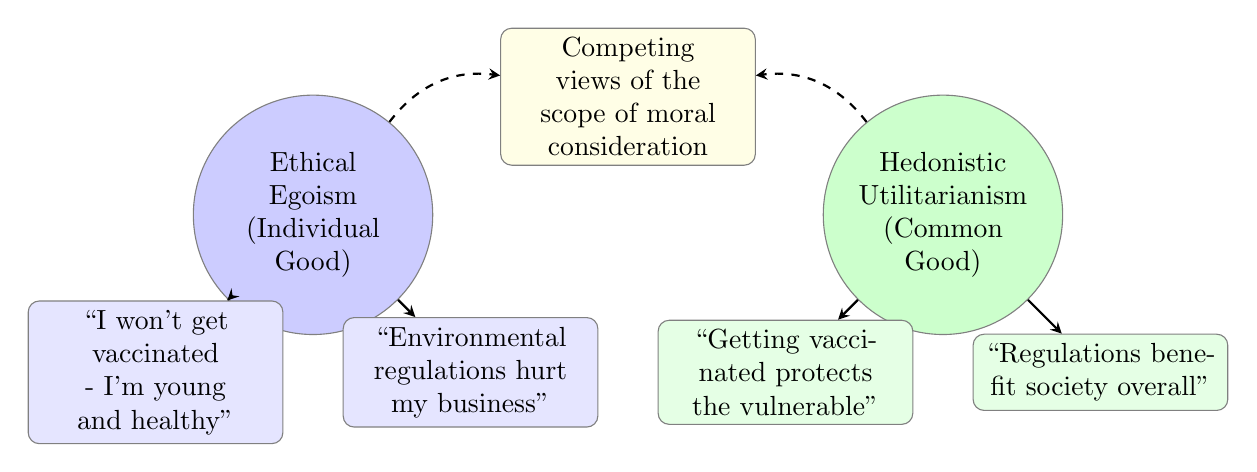
\begin{tikzpicture}[
        concept/.style={circle, draw=black!50, minimum size=2.5cm, text width=2.2cm, text centered},
        example/.style={rectangle, rounded corners, draw=black!50, text width=3cm, align=center},
        arrow/.style={->, >=stealth, thick}
    ]
        % Main concepts
        \node[concept, fill=blue!20] (egoism) at (-4,0) {Ethical Egoism\\(Individual Good)};
        \node[concept, fill=green!20] (utilitarian) at (4,0) {Hedonistic Utilitarianism\\(Common Good)};
        
        % Relationship between them
        \node[example, fill=yellow!10] (relation) at (0,1.5) 
            {Competing views of the scope of moral consideration};
        \draw[arrow, dashed, bend left] (egoism) to (relation);
        \draw[arrow, dashed, bend right] (utilitarian) to (relation);
        
        % Examples for Ethical Egoism
        \node[example, fill=blue!10] (ego_ex1) at (-6,-2) 
            {``I won't get vaccinated - I'm young and healthy''};
        \node[example, fill=blue!10] (ego_ex2) at (-2,-2) 
            {``Environmental regulations hurt my business''};
            
        % Examples for Utilitarianism
        \node[example, fill=green!10] (util_ex1) at (2,-2) 
            {``Getting vaccinated protects the vulnerable''};
        \node[example, fill=green!10] (util_ex2) at (6,-2) 
            {``Regulations benefit society overall''};
            
        % Connections
        \draw[arrow] (egoism) -- (ego_ex1);
        \draw[arrow] (egoism) -- (ego_ex2);
        \draw[arrow] (utilitarian) -- (util_ex1);
        \draw[arrow] (utilitarian) -- (util_ex2);
        
    \end{tikzpicture}
    \end{center}
\end{frame}

\begin{frame}{Problems with Bentham's View}
    \begin{itemize}
        \item The \textbf{quantification problem}: Bentham's felicific calculus assumes we can measure and compare different types of pleasure and pain with precision, but how do we really compare the pleasure of eating ice cream with the pleasure of reading poetry?
        
        \item The \textbf{aggregation problem}: Simply adding up pleasures and pains across individuals ignores questions of justice and fair distribution—should we sacrifice one person's fundamental rights to produce slightly more happiness for many others?
        
        \item The \textbf{motivation problem}: Bentham's psychological hedonism (that pleasure and pain are the only motives for action) seems to conflict with other types of human "goods" (such as knowledge, friendship, etc.).
        
        \item The \textbf{complexity problem}: The felicific calculus becomes impossibly complex when we try to account for all consequences of actions across time and space—illustrated by contemporary challenges in climate policy and artificial intelligence governance.
        
        \item These critiques led to important refinements in utilitarian theory, particularly Mill's qualitative distinction between higher and lower pleasures.
    \end{itemize}
\end{frame}

\begin{frame}{John Stuart Mill: Biography (1806-1873)}
    \begin{itemize}
        \item Mill's early life represented an experiment in \textbf{utilitarian education}, as his father James Mill and Jeremy Bentham designed an intensive educational program to create a philosophical prodigy, teaching him Greek at three and economics by age thirteen.
        
        \item His mental crisis at age twenty led him to question pure Benthamite rationalism, discovering through poetry and art that human happiness requires both intellectual and emotional development—a insight central to his later philosophical work.
        
        \item As a public intellectual, Mill worked at the East India Company while writing influential works on logic, economics, and political theory, including \textit{Principles of Political Economy} (1848) and \textit{On Liberty} (1859).
        
        \item Mill's career as a social reformer in Parliament (1865-1868) demonstrated his commitment to practical applications of utilitarian principles, especially in promoting women's suffrage and workers' rights.
    \end{itemize}
\end{frame}

\begin{frame}{Harriet Taylor Mill: Biography (1807-1858)}
    \begin{itemize}
        \item Harriet Taylor Mill developed sophisticated utilitarian arguments for equality, particularly in her essay "The Enfranchisement of Women" (1851), which argued that social progress requires developing the talents of all individuals regardless of gender.
        
        \item Her concept of cooperative social progress emphasized how equality and individual development contribute to collective welfare, influencing both feminist theory and democratic socialism.
        
        \item The Mills' intellectual partnership challenged Victorian conventions about gender roles while demonstrating their philosophical commitment to judging actions by consequences rather than social rules.
        
        \item Her work on \textbf{economic justice} argued that worker cooperatives and profit-sharing could align individual and collective interests—ideas that continue to influence discussions of workplace democracy and economic inequality.
    \end{itemize}
\end{frame}

\begin{frame}{Mill's Utilitarianism: Theory}
    \begin{itemize}
        \item Mill introduced the crucial distinction between \textbf{higher} and \textbf{lower pleasures}, arguing that some forms of happiness are inherently more valuable because they engage our uniquely human capacities for intellectual and moral development.
        
        \item His concept of \textbf{competent judges}—those who have experienced both types of pleasure—provides a method for establishing qualitative differences: "It is better to be Socrates dissatisfied than a fool satisfied."
        
        \item Mill developed \textbf{indirect utilitarianism}, arguing that utility is often best served by following general rules and protecting individual rights rather than calculating the consequences of each action.
        
        \item His \textbf{harm principle} states that power can only be rightfully exercised over individuals to prevent harm to others—a principle that continues to influence debates about personal freedom versus collective welfare.
        
    \end{itemize}
\end{frame}
\begin{frame}{Mill's Utilitarianism: Practical Applications}
    \begin{itemize}
        \item Mill developed powerful \textbf{antislavery arguments} based on utility, contending that slavery not only directly harmed its victims but corrupted the moral character of slave-owners and society at large—showing how utilitarian thinking supports fundamental human rights.
        
        \item His groundbreaking work \textbf{"The Subjection of Women"} (1869) argued that gender equality would dramatically increase human welfare by developing women's talents and improving relationships between men and women—ideas that helped launch the feminist movement.
        
        \item In economics, Mill advocated for \textbf{progressive taxation}, \textbf{worker cooperatives}, and limits on inheritance to reduce inequality. He argued that free markets should serve human welfare rather than being ends in themselves—principles still debated in discussions of economic justice.
        
        \item As a Member of Parliament, Mill championed \textbf{proportional representation}, arguing that true democracy requires protecting minority viewpoints and ensuring all groups have a political voice—anticipating contemporary debates about electoral reform.
        
    \end{itemize}
\end{frame}

\begin{frame}{Making Decisions Using Act Utilitarianism}
    \begin{center}
    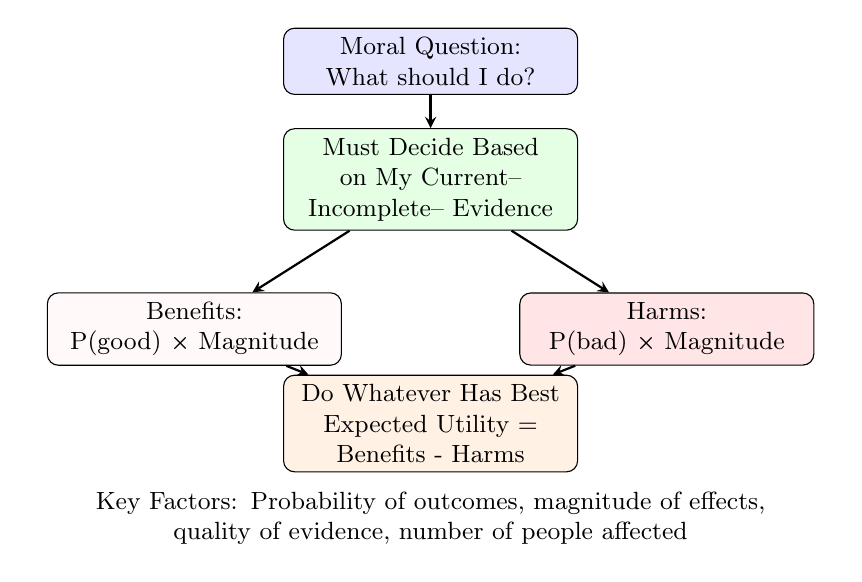
\begin{tikzpicture}[
        block/.style={rectangle, draw, rounded corners, text width=3.5cm, minimum height=0.7cm, 
            align=center, font=\small},
        arrow/.style={->, >=stealth, thick}
    ]
        % Start with moral question
        \node[block, fill=blue!10] (start) at (0,1) {Moral Question: What should I do?};
        
        % Evidence and outcomes
        \node[block, fill=green!10] (evidence) at (0,-0.5) 
            {Must Decide Based on My Current--Incomplete-- Evidence};
            
        % Benefits analysis
        \node[block, fill=pink!10] (benefits) at (-3,-2.4) 
            {Benefits:\\P(good) × Magnitude};
            
        % Harms analysis    
        \node[block, fill=red!10] (harms) at (3,-2.4) 
            {Harms:\\P(bad) × Magnitude};
            
        % Final calculation
        \node[block, fill=orange!10] (calculate) at (0,-3.6) 
            {Do Whatever Has Best Expected Utility =\\Benefits - Harms};
            
        % Connect everything
        \draw[arrow] (start) -- (evidence);
        \draw[arrow] (evidence) -- (benefits);
        \draw[arrow] (evidence) -- (harms);
        \draw[arrow] (benefits) -- (calculate);
        \draw[arrow] (harms) -- (calculate);
        
        % Add key considerations in text
        \node[text width=10cm, align=center, font=\small] at (0,-4.8) 
            {Key Factors: Probability of outcomes, magnitude of effects,\\
            quality of evidence, number of people affected};
    \end{tikzpicture}
    \end{center}
\end{frame}

\begin{frame}{Contemporary Utilitarianism: From Sidgwick to Singer}
    \begin{itemize}
        \item \textbf{Henry Sidgwick} (1838-1900) offered sophisticated defenses of utilitarianism in his work \textit{The Methods of Ethics}, developing the concept of \textbf{rational benevolence} as the foundation for impartial consideration of everyone's welfare.
        
        \item \textbf{R.M. Hare} (1919-2002) developed \textbf{preference utilitarianism}, which measures utility in terms of preference satisfaction rather than mental states like pleasure—allowing utilitarianism to better handle cases involving unconscious beings or future persons.
        
        \item \textbf{Derek Parfit} (1942-2017) explored how utilitarianism addresses questions of \textbf{personal identity} and \textbf{future generations}, showing how our ordinary moral intuitions often fail when dealing with large numbers or long time scales.
        
        \item \textbf{Peter Singer} (1946-) has applied utilitarian reasoning to practical ethics, developing influential arguments about \textbf{animal welfare}, \textbf{global poverty}, and \textbf{effective altruism} that have sparked real-world movements for change.
    \end{itemize}
\end{frame}

\section{Thought Experiements and Objections}
\begin{frame}{Thought Experiments and Objections}
    \begin{itemize}
        \item Thought experiments are hypothetical scenarios designed to test moral intuitions and challenge ethical theories—often revealing tensions or contradictions in our moral beliefs.
        
        \item Utilitarianism has been the subject of many famous thought experiments that highlight key problems and objections to the theory, including the Trolley Problem, the Drowning Child, and the Experience Machine.
        
        \item These cases raise questions about the demandingness of utilitarian ethics, the role of personal integrity in moral decision-making, and the relationship between individual rights and aggregate welfare.
        
        \item By examining these thought experiments, we can better understand the strengths and limitations of utilitarianism as a moral theory and how it applies to real-world ethical dilemmas.
    \end{itemize}
\end{frame}

\begin{frame}{The Trolley Problem (Philippa Foot, 1967)}
    \begin{quote}
        A runaway trolley is heading towards five people tied to the tracks. You can pull a lever to divert it to another track, but doing so will kill one person tied to that track. What should you do?
    \end{quote}
    \begin{itemize}
        \item This thought experiment highlights key tensions in utilitarian thinking:
        
        \item From an act utilitarian perspective, the choice seems clear: divert the trolley to save net four lives.
        
        \item However, this raises troubling questions about actively causing death versus allowing death to occur—challenging the distinction between acts and omissions that many moral theories rely upon.
        
        \item Modern variations (like the "fat man" version where you must push someone onto the tracks) reveal how our moral intuitions often conflict with straightforward utilitarian calculations.
    \end{itemize}
\end{frame}

\begin{frame}{The Drowning Child (Peter Singer, 1972)}
    \begin{quote}
        "If I am walking past a shallow pond and see a child drowning in it, I ought to wade in and pull the child out. This will mean getting my clothes muddy, but this is insignificant compared to the death of the child."
    \end{quote}
    \begin{itemize}
        \item Singer uses this example to argue that physical distance and nationality are morally irrelevant—if we accept an obligation to save a drowning child nearby, we should also help distant children dying of poverty.
        
        \item The thought experiment challenges our intuitions about moral distance and special obligations to those near us. 
        
        \item It raises questions about the demandingness of utilitarian ethics: if we should save one child at little cost to ourselves, shouldn't we keep giving until the marginal utility of our money equals that of recipients? (Many people find this conclusion difficult to swallow.)
        
        \item This argument helped launch the effective altruism movement and continues to influence debates about global poverty and moral obligations.
    \end{itemize}
\end{frame}

\begin{frame}{The Experience Machine (Robert Nozick, 1974)}
    \begin{quote}
        Suppose there were an experience machine that would give you any experience you desired. Would you plug in for life, preprogramming your life's experiences?
    \end{quote}
    \begin{itemize}
        \item This thought experiment challenges hedonistic utilitarianism by suggesting that we value things beyond just experiences and mental states.
        
        \item Nozick argues that most people would refuse to plug in because:
            \begin{itemize}
                \item We want to actually do things, not just have the experience of doing them
                \item We want to be certain kinds of people, not just collections of experiences
                \item We want to connect with reality, not live in an artificial simulation
            \end{itemize}
        
        \item This suggests that preference utilitarianism might better capture what we truly value than purely hedonistic approaches.
    \end{itemize}
\end{frame}

\begin{frame}{George the Chemist (Bernard Williams, 1973)}
    \begin{quote}
        George, a chemist, is offered a job developing chemical weapons. If he refuses, someone else will take the position and develop even worse weapons. Should he take the job?
    \end{quote}
    \begin{itemize}
        \item This case illustrates Williams's critique that utilitarianism can alienate us from our deepest moral convictions and personal integrity.
        
        \item A strict utilitarian calculation suggests George should take the job to prevent worse outcomes—but this seems to ignore the moral cost of compromising one's fundamental values.
        
        \item The example raises questions about:
            \begin{itemize}
                \item The role of personal moral integrity in ethical theory
                \item Whether utilitarian calculations can capture all morally relevant factors
                \item How to weigh individual moral agency against aggregate consequences
            \end{itemize}
    \end{itemize}
\end{frame}

\begin{frame}{The Repugnant Conclusion (Derek Parfit, 1984)}
    \begin{itemize}
        \item Derek Parfit's Repugnant Conclusion thought experiment asks us to compare two possible populations:
            \begin{itemize}
                \item Population A: 10 billion people with very high quality of life (Z)
                \item Population B: 100 billion people with lives barely worth living (A)
            \end{itemize}
        \item Parfit shows that total utilitarianism leads to the conclusion that a very large population with lives barely worth living (Z) would be better than a smaller population with very high quality of life (A).
        
        \item This seems to conflict with our moral intuitions and raises deep questions about population ethics:
            \begin{itemize}
                \item How do we compare different-sized populations?
                \item Is there value in the mere addition of lives barely worth living?
                \item Should we focus on total or average utility?
            \end{itemize}
    \end{itemize}
\end{frame}


\begin{frame}{Comparing the Thought Experiments}
    \begin{itemize}
        
        \item These thought experiments highlight different challenges for utilitarian theory:
        
        \item \textbf{Action vs. Omission}: The Trolley Problem questions whether actively causing harm is different from allowing it to happen.
        
        \item \textbf{Demandingness}: Singer's Drowning Child reveals how utilitarian ethics might require significant personal sacrifice.
        
        \item \textbf{Value Beyond Experience}: Nozick's Experience Machine suggests we care about more than just mental states.
        
        \item \textbf{Personal Integrity}: Williams's George shows how utilitarian calculations might conflict with personal moral convictions.
        
        \item \textbf{Population Ethics}: Parfit's Repugnant Conclusion exposes paradoxes in how we value different possible populations.
    \end{itemize}
\end{frame}

\section{Variations in Utilitarian Thought}
\begin{frame}{Variations in Utilitarian Thought}
    \begin{itemize}
        \item Utilitarianism has evolved into a diverse family of theories that address different challenges and applications, including act vs. rule utilitarianism, hedonistic vs. preference utilitarianism, total vs. average utilitarianism, and maximizing vs. satisficing approaches.
        
        \item These variations reflect the ongoing debate about how best to balance individual welfare with collective interests, personal rights with social obligations, and short-term gains with long-term consequences.
        
        \item By exploring these different approaches, we can better understand the strengths and limitations of utilitarianism as a moral theory and how it applies to contemporary ethical dilemmas.
        
        \item These debates have practical implications for policy decisions in areas like global poverty, public health, animal welfare, and future risks—highlighting the importance of ethical theory in guiding real-world choices.
    \end{itemize}

\end{frame}

\begin{frame}{Act vs. Rule Utilitarianism}
    % R.M. Hare defended rule utilitarianism
    \begin{itemize}
        \item \textbf{Act utilitarianism} evaluates each action independently, requiring us to calculate consequences every time we act. Endorsed by Peter Singer, who argues this leads to more precise ethical decisions in cases like charitable giving and animal welfare.
        
        \item \textbf{Rule utilitarianism} judges actions by rules that would create the best outcomes if universally followed. Richard Hare argued this approach better matches our moral intuitions and provides more reliable guidance for everyday moral decisions.
        
        \item This distinction emerged from attempts to address the practical challenges of constant utilitarian calculation, particularly in time-sensitive situations where detailed analysis is impossible.
        
        \item The debate mirrors the broader tension between \textbf{situational ethics} and \textbf{universal moral rules} in ethical theory, similar to disputes between particularists and generalists in moral philosophy.
    \end{itemize}
 \end{frame}
 
 \begin{frame}{Hedonistic vs. Preference Utilitarianism}
    % Key debate in modern utilitarian thought
    \begin{itemize}
        \item \textbf{Hedonistic utilitarianism} focuses purely on pleasure and pain as moral currency. Jeremy Bentham developed this view, arguing all pleasures are qualitatively similar, though John Stuart Mill later introduced the concept of "higher" and "lower" pleasures.
        
        \item \textbf{Preference utilitarianism} considers the satisfaction of informed desires instead. R.M. Hare pioneered this approach to better handle complex cases like posthumous wishes and unconscious patients' previously stated preferences.
        
        \item The distinction matters especially in medical ethics and animal welfare debates, where questions of consciousness and preference satisfaction become critically important for decision-making.
        
        \item Modern neuroscience research on \textbf{subjective well-being} has added new dimensions to this classic debate, particularly through studies of happiness metrics and neural correlates of pleasure.
    \end{itemize}
 \end{frame}
 
 \begin{frame}{Total vs. Average Utilitarianism}
    % Contemporary population ethics
    \begin{itemize}
        \item \textbf{Total utilitarianism} aims to maximize the sum of welfare across all individuals. Henry Sidgwick defended this view while acknowledging its challenging implications, including Derek Parfit's famous \textbf{Repugnant Conclusion}.
        
        \item \textbf{Average utilitarianism} focuses on maximizing the mean welfare level instead. Developed by Hardin as a response to population ethics paradoxes, though it faces its own challenges with the "mere addition paradox."
        
        \item This debate shapes how we think about future generations and population policy, particularly in discussions of climate change mitigation and resource allocation between generations.
        
        \item The emergence of \textbf{longtermism} as a philosophical movement has given new relevance to these population ethics questions, especially in discussions of existential risk and humanity's cosmic endowment.
    \end{itemize}
 \end{frame}
 
 \begin{frame}{Maximizing vs. Satisficing}
    % Modern development in utilitarian theory
    \begin{itemize}
        \item \textbf{Maximizing utilitarianism} requires achieving the absolute best outcome possible. Peter Singer exemplifies this demanding approach in his work on effective altruism, arguing we should give until the marginal utility of our money equals that of recipients.
        
        \item \textbf{Satisficing utilitarianism} accepts any outcome above a sufficient threshold. Michael Slote introduced this concept to make utilitarianism more psychologically realistic, acknowledging the costs of constant optimization.
        
        \item This distinction helps us understand the practical limits of moral obligations, particularly in contexts where decision costs and cognitive burden become significant factors.
        
        \item The rise of the \textbf{effective altruism movement} has renewed interest in the psychological feasibility of maximizing approaches, while suggesting practical compromises between maximizing and satisficing through concepts like "earning to give."
    \end{itemize}
 \end{frame}



\begin{frame}{Application: Global Poverty and Effective Altruism}
    \begin{itemize}
        \item Contemporary utilitarians argue that we have strong moral obligations to help the global poor because we can save lives at relatively low cost to ourselves—for example, providing malaria nets or deworming treatments can save a life for a few thousand dollars.
        
        \item The \textbf{effective altruism} movement applies utilitarian reasoning to charitable giving, using evidence and analysis to identify the most cost-effective ways to do good—leading to organizations like GiveWell that evaluate charities' impact per dollar.
        
        \item This approach challenges traditional ideas about charity by suggesting we should donate based on effectiveness rather than emotional connection, leading to debates about \textbf{cause prioritization} between areas like global health, animal welfare, and existential risk.
        
        \item Critics argue this approach is too coldly calculating, but utilitarians respond that being more effective at helping others is the truly compassionate choice—noting that sentimental giving often fails to maximize positive impact.
    \end{itemize}
\end{frame}

\begin{frame}{Application: Animal Welfare and Factory Farming}
    \begin{itemize}
        \item Utilitarians argue that the capacity to suffer, not species membership, determines moral status—meaning that factory farming creates massive amounts of suffering that we are morally obligated to prevent.
        
        \item Contemporary research on \textbf{animal consciousness} and \textbf{pain perception} strengthens these arguments by showing that animals experience rich emotional lives and can suffer in ways similar to humans—making their welfare a pressing moral concern.
        
        \item The scale of factory farming (over 70 billion land animals killed annually) makes this potentially one of the largest sources of suffering in the world from a utilitarian perspective, leading to arguments for vegetarianism and support for alternative proteins.
        
        \item This application shows how utilitarian thinking can lead to radical conclusions by following the logic of minimizing suffering consistently—challenging common practices we often take for granted.
    \end{itemize}
\end{frame}

\begin{frame}{Singer on the "Expanding Circle"}
\begin{quote}
    In an earlier stage of our development most human groups held to a tribal ethic. Members of the tribe were protected, but people of other tribes could be robbed or killed as one pleased. Gradually the circle of protection expanded, but as recently as 150 years ago we did not include blacks. So African human beings could be captured, shipped to America, and sold. In Australia white settlers regarded Aborigines as a pest and hunted them down, much as kangaroos are hunted down today. Just as we have progressed beyond the blatantly racist ethic of the era of slavery and colonialism, so we must now progress beyond the speciesist ethic of the era of factory farming, of the use of animals as mere research tools, of whaling, seal hunting, kangaroo slaughter, and the destruction of wilderness. We must take the final step in expanding the circle of ethics.
\end{quote}
-- Peter Singer
\end{frame}

\begin{frame}{Contemporary Applications of Utilitarian Analysis}
    \begin{table}[]
        \scriptsize
        \begin{tabular}{p{2.2cm}p{3.5cm}p{3.5cm}}
            \textbf{Domain} & \textbf{Key Issues} & \textbf{Utilitarian Approach} \\\hline
            
            Global Poverty & \begin{itemize}\setlength\itemsep{0em}
                \item Extreme poverty
                \item Economic development
                \item Aid effectiveness
            \end{itemize} & 
            Maximize welfare per dollar through evidence-based interventions (e.g., direct cash transfers, deworming programs, malaria prevention) \\\hline
            
            Public Health & \begin{itemize}\setlength\itemsep{0em}
                \item Healthcare rationing
                \item Vaccine distribution
                \item Research priorities
            \end{itemize} & 
            Allocate resources to maximize QALYs (Quality-Adjusted Life Years), prioritizing interventions with greatest impact per cost \\\hline
            
            Animal Welfare & \begin{itemize}\setlength\itemsep{0em}
                \item Factory farming
                \item Wild animal suffering
                \item Research ethics
            \end{itemize} & 
            Consider welfare of all sentient beings; focus on scale of suffering in industrial agriculture and potential interventions \\\hline
            
            Future Risks & \begin{itemize}\setlength\itemsep{0em}
                \item Climate change
                \item AI safety
                \item Existential risk
            \end{itemize} & 
            Account for long-term effects and potential impacts on future generations; emphasize prevention of catastrophic risks \\\hline
            
            Medical Ethics & \begin{itemize}\setlength\itemsep{0em}
                \item End-of-life care
                \item Organ allocation
                \item Triage decisions
            \end{itemize} & 
            Balance quality of life, patient autonomy, and resource allocation; consider both current and future welfare
        \end{tabular}
    \end{table}
\end{frame}



\begin{frame}{Wrap Up: Key Themes in Utilitarian Thought}
    In examining utilitarianism from its classical foundations through its contemporary applications, several key themes emerge that help us understand both its enduring appeal and its challenges:
    
    \begin{itemize}
        \item The persistent tension between impartial welfare maximization and our intuitions about justice, rights, and special obligations shows how utilitarianism pushes us to examine our moral assumptions.
        
        \item The evolution from Bentham's hedonistic calculus to modern frameworks like QALYs demonstrates how utilitarian thinking drives the development of practical tools for ethical decision-making.
        
        \item Contemporary applications in areas like effective altruism show how utilitarian principles can guide concrete actions while raising challenging questions about moral demands.
        
        \item The ongoing debate between different versions of utilitarianism (act vs. rule, hedonistic vs. preference) reflects broader questions about how to balance systematic ethical thinking with practical reality.
    \end{itemize}
\end{frame}

\begin{frame}{Discussion Questions, Part 1}
    Consider these questions about utilitarianism's theoretical foundations:
    \begin{itemize}
        \item Imagine you're a hospital administrator deciding how to allocate scarce medical resources. How would different versions of utilitarianism (hedonistic, preference, rule) approach this decision? What factors would each consider most important?
        
        \item Bernard Williams argues that utilitarianism alienates us from our personal projects and relationships. Consider a case where maximizing utility would require abandoning a close friend in need. How might a utilitarian respond to this criticism?
        
        \item Examine the claim that we can't reliably predict the long-term consequences of our actions. Does this undermine utilitarianism as a practical ethical framework? How might different types of utilitarianism handle this challenge?
        
        \item Looking at Mill's distinction between higher and lower pleasures, are there meaningful ways to compare qualitatively different experiences? What criteria might we use?
    \end{itemize}
\end{frame}

\begin{frame}{Discussion Questions, Part 2}
    Explore these questions about contemporary applications:
    \begin{itemize}
        \item Peter Singer argues that we have strong obligations to help the global poor. Consider your own consumption choices: how would strict utilitarian reasoning change your lifestyle? Is such demanding morality sustainable?
        
        \item Analyze factory farming through different utilitarian lenses (hedonistic vs. preference, act vs. rule). How do different approaches weigh economic benefits against animal welfare? What policies would each version support?
        
        \item Consider autonomous vehicles programmed with utilitarian decision-making principles. Should they prioritize minimizing total casualties even if that means sometimes sacrificing their passengers? What does this tell us about utilitarianism and individual rights?
        
        \item How should utilitarians weigh present versus future welfare? Consider cases like climate change or AI development where actions today could affect millions of future lives.
    \end{itemize}
\end{frame}



\end{document}